\chapter{Drone Component Comparisons}
%\addcontentsline{toc}{chapter}{Introduction}\label{Introduction}

In this section different component of the drone will be discussed. The components discussed are those involved in the construction of the basic drone, before any mine specific sensors are added.
\newline
\href{https://oscarliang.com/fpv-drone-guide/#Basic-Drone-Control}{\textcolor{blue}{\underline{Drone Basics}}}
\section{Frame}
	Frame
	\begin{itemize}
		\item \href{https://www.team-blacksheep.com/products/prod:sourceone_v5}{\textcolor{blue}{\underline{Source One V5}}}: Affordable, open-source, compatible with latest hardware, large collection of spare parts, mods and accessories ("check \href{https://www.thingiverse.com/}{\textcolor{blue}{\underline{Thingyverse}}} website"), 123.5g
		\item \href{https://shop.iflight.com/AOS5-V5-Frame-Kit-Pro2127?search=aos}{\textcolor{blue}{\underline{AOS 5 V2}}}: FPV performance focussed, exceptional noise performance and prop wash handling, complex building and repairing, arms are prone to damage during crashes, 125g
	\end{itemize}
	\underline{Decision: Source One V5}
	

\section{Motors and Propellers}
	\subsection{Motor Considerations}
		\begin{itemize}
			\item Lower KV ratings for better efficiency
			\item Larger LiPo or Li-ion Batteries
		\end{itemize}
	\href{https://shop.iflight.com/R5-2207-2050KV-FPV-motor-Pro2029?search=R5%202207}{\textcolor{blue}{\underline{iFlight R5 2207 2050KV FPV motor}}} (Higher efficiency at low revs and higher max payload)\newline
	\href{https://store.tmotor.com/product/F60pro4-v2-kv1750-fpv-motor.html}{\textcolor{blue}{\underline{T-Motor F60PRO IV V2.0 Fpv Racing Drone Motor 4-6S KV1750 (RMF-Owl)}}}\newline
	\href{https://store.tmotor.com/product/f40pro-4-fpv-motor.html}{\textcolor{blue}{\underline{T-Motor F40PRO IV Fpv Racing Drone Motor 4-6S KV1950/KV2400}}}\newline
	\href{https://store.tmotor.com/product/f60prov-fpv-motor.html}{\textcolor{blue}{\underline{T-Motor F60PROV 2207.5 Fpv Racing Drone Motor 4-6S KV1750/KV1950/KV2020/KV2550}}}\newline
	\newline
	\underline{Decision: iFlight R5 2207 2050KV FPV motor}

	\subsection{Propeller Considerations}
		\begin{itemize}
			\item Lower pitch propeller for better efficiency
			\item 5" = smaller, 7" more payload and better efficiency
			\item Therefore 6" might be optimal, but not commonly available
			\item Props can produce 20-30\% less thrust in air compared to static thrust test
			\item Use Props suggested by motor manufacture, to achieve results similar to those in the motor test reports
		\end{itemize}
	\href{https://goblinhobbies.co.za/fpv/props/5/gemfan-51466-mck-v2-3-blade-propellers-5-0mm-shaft-4pcs.html}{\textcolor{blue}{\underline{Gemfan 51466 MCK V2 3-Blade Propellers (5.0mm Shaft 4PCS)}}} SA\newline
	\href{https://store.tmotor.com/product/t5146-fpv-propeller.html}{\textcolor{blue}{\underline{T5146}}}\newline	
	\href{https://www.gemfanhobby.com/list.aspx?cid=20}{\textcolor{blue}{\underline{Gemfan 51466, 51477, 51499, 5149}}}\newline	
	\href{https://shop.robitronic.com/en/azure-5150-tri-blade-prop-az51500303}{\textcolor{blue}{\underline{Azure 5150 Tri-Blade Prop Polestar}}}\newline	
	\href{https://azurepowerusa.com/collections/5-inch-props}{\textcolor{blue}{\underline{Azure Blades 5140, 5148, 5150}}}\newline
	\newline
	\underline{Decision: Gemfan 51466 MCK V2 RACING PROPS (From Gemfan website)}\newline
	\underline{Decision also to test: Gemfan Hulkie 5055S-3 and Gemfan Hurricane 51499-3 (From Gemfan website)}

\section{Electric Speed Controller (ESC)}
	\href{https://robocraze.com/blogs/post/how-to-choose-esc-for-quadcopter}{\textcolor{blue}{\underline{Considerations}}}:
	\begin{enumerate}
		\item The current rating / ampere rating is the first thing to consider. make sure ESC can can handle max amount of current that motors can draw. Look at continuous and burst(e.g. 10 sec) current rating.
		\item Input Voltage rating. Check that it is 6s compatible; preferably 4S-6S.
		\item ESC Firmware
		\begin{itemize}
			\item Popular firmware = BLHeli\_S or BLHeli\_32 (99\% of FPV's)
			\item Firmware: BLHeli\_32 Is faster and more future proof
			\item Protocol: Multishot, DShot300 and DShot600 (number is speed of controller), ProShot
		\end{itemize}
		\item ECS Processor: Support different firmware
		\item Consider power needs of motors
		\item ESC may need specific firmware installed from flight controller, so check compatibility.
	\end{enumerate}
	

\section{Flight Controller/Autopilot}
\href{https://oscarliang.com/flight-controller-explained/}{\textcolor{blue}{\underline{Flight Controllers Explained}}}
	
Considerations:
	\begin{itemize}
		\item Popular firmware
			\begin{enumerate}
				\item Betaflight
					\begin{itemize}
						\item open source
						\item performs well
						\item updated frequently
						\item huge selection of flight controllers available
						\item added features for long-range flights
						\item lots of resources available online
						\item Best Hardware support
						\item Best For Beginners
						\item HOWEVER, Mainly used in FPV style drones and not made for autonomous drones
					\end{itemize}
				\item Emuflight
					\begin{itemize}
						\item Try when Betaflight is not working, runs on same hardware
					\end{itemize}
				\item ArduPilot
					\begin{itemize}
						\item Emphasis on versatility and community support
						\item Wide Range of Supported Platforms
						\item Extensive Documentation
						\item User-Friendly Configuration: ArduPilot features a user-friendly ground control station (GCS) called Mission Planner. This interface simplifies the process of configuring the flight stack and planning missions.
						\item Supports a variety of vehicles, including quadcopters, planes, rovers, 
						\item Often used in autonomous vehicles
					\end{itemize}
				\item INAV
					\begin{itemize}
						\item Good at autonomous flight, after ArduPilot
					\end{itemize}
				\item PX4 \href{https://www.thedroningcompany.com/blog/px4-vs-ardupilot-choosing-the-right-open-source-flight-stack}{\textcolor{blue}{\underline{1}}}
					\begin{itemize}
						\item Emphasis on precision, reliability, and modularity
						\item PX4 boasts advanced autopilot capabilities, including support for many flight modes, obstacle avoidance, and GPS-denied navigation
						\item Suitable for surveying, mapping, and search and rescue missions
						\item Its reputation for stability and precision has made it a preferred choice for companies seeking reliable drone solutions
						\item If you need precise control and advanced autonomous capabilities, PX4 may be the better choice
						\item If you have specific requirements that necessitate custom software modules or sensor integrations, PX4's modular architecture might be more appealing.
					\end{itemize}
						\underline{Decision: PX4}
			\end{enumerate}
		\item all have gyroscope, accelerometer
		\item only some have barometer and compass(magnetometer)(Not necessary)
		\item can also serve as hub for  ESC, GPS, LED, servos, radio receiver, FPV cam and VTX
		\item Make sure flight controller has soft mount, increases performance
		\item Check Gyro specs. 
			\begin{itemize}
				\item Avoid or thoroughly research the following:
					\begin{itemize}
						\item MPU6500
						\item MPU9250
						\item ICM20689
						\item ICM20602
					\end{itemize}
				\item Rather try:
					\begin{itemize}
						\item MPU6000
						\item BMI270
					\end{itemize}
			\end{itemize}
		\item 
		\href{https://oscarliang.com/f1-f3-f4-flight-controller/}{\textcolor{blue}{\underline{STM Chip naming convention}}}
	\end{itemize}

	\href{https://store.cuav.net/shop/cuav-v6x/}{\textcolor{blue}{\underline{CUAV}}}
	\href{https://holybro.com/products/pixhawk-6x?variant=42471703085245}{\textcolor{blue}{\underline{holybro}}}


\section{Microcontroller}
	YYY
	
	YYY:
	
	\begin{itemize}
		\item YYY
		\item YYY
		\item YYY
	\end{itemize}

	Here are some of the images :

	\begin{figure}[H]
		\centering
		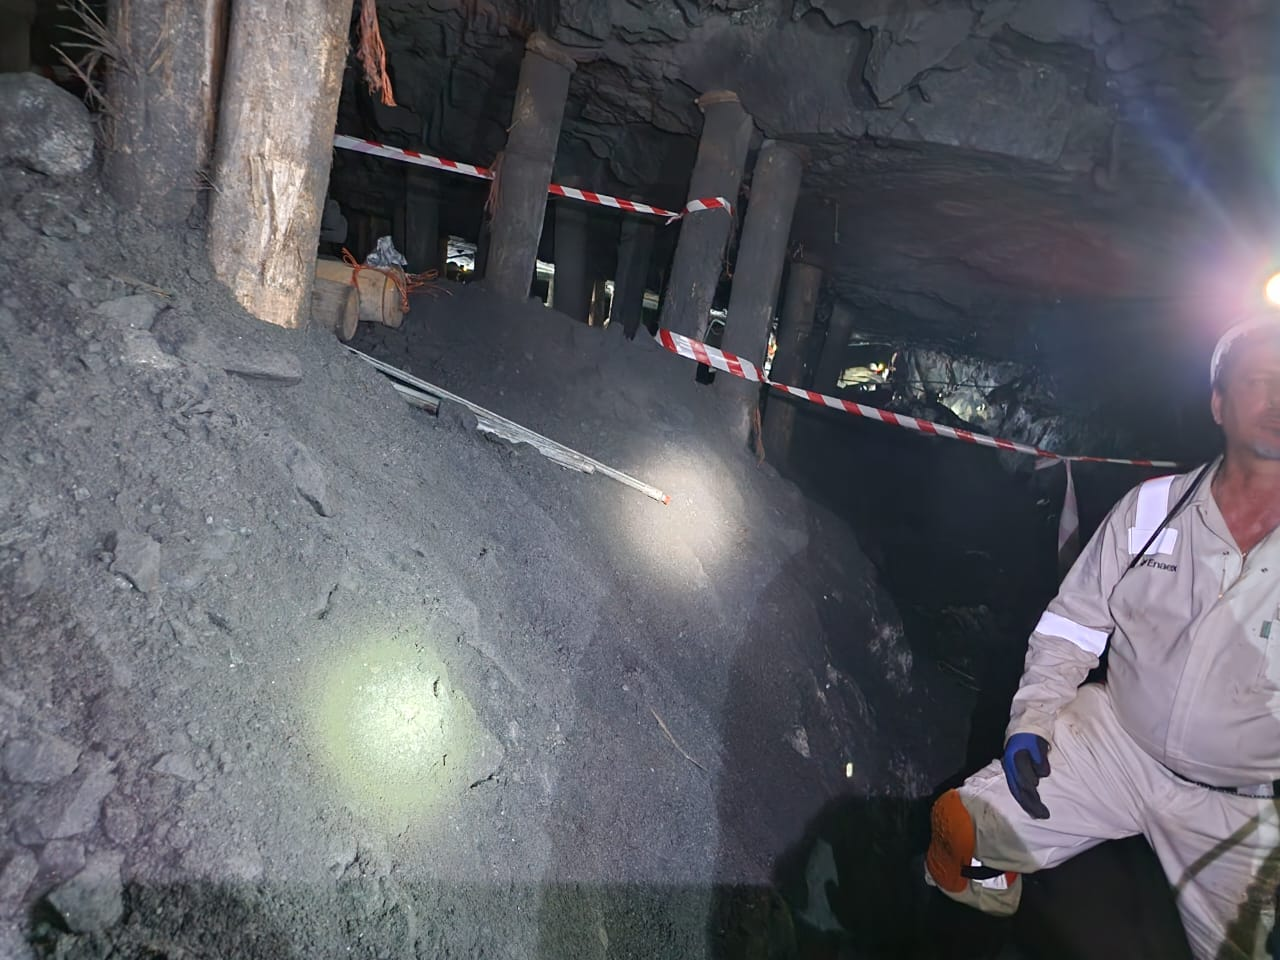
\includegraphics[width=0.7\linewidth]{Images/Impala1}
		\caption{Impala platinum mine. Person for scale, on the left is the narrow reef, which is less than 1m in height. Note the rise between the walkway and the reef that is being mined. The wooden pillars are there to support the roof.}
		\label{fig:Impala1}
	\end{figure}

	
\section{Power Distribution Board (PDB)}
	

\section{Battery}
\href{https://www.unmannedsystemstechnology.com/feature/lipo-vs-lithium-ion-batteries-for-unmanned-robotics-applications/#:~:text=When%20deciding%20on%20a%20battery,probably%20the%20way%20to%20go.}{\textcolor{blue}{\underline{LiPo vs. Li-ion}}}
	\begin{enumerate}
		\item LiPo
		Pros:
		\begin{itemize}
			\item Performance focussed
			\item Holds highest voltage under load - perform well in amp draw applications
			\item Come in many different form factors
			\item Maintains lower temperatures under high discharge
		\end{itemize}
		Cons:
		\begin{itemize}
			\item More prone to thermal runaway when punctured or damaged
			\item Batteries provide around half the life cycles of a Li-Ion
			\item Can be discharged down to 3v per cell
		\end{itemize}
		\item Li-ion
		Pros:
		\begin{itemize}
			\item Endurance focussed
			\item High energy density for longer runtime and lighter weight
			\item Safer than liPo because of the metal enclosure
		\end{itemize}
		Cons:
		\begin{itemize}
			\item Only come in cylindrical shapes with specific sizes which can create some limitations to fit in certain applications
			\item In high amp draw applications, they will have lower voltage under load compared to LiPo
			\item Tend to hold higher temperatures during and especially after performing a higher discharge rate
		\end{itemize}
	\end{enumerate}
	Decision: Use LiPo as lots of components that could be drawing high loads
	Considerations:


	\href{https://oscarliang.com/6s-mini-quad-racing-drone/#:~:text=A%206S%20LiPo%20battery%20has,LOWER%20amp%20draw}{\textcolor{blue}{\underline{4S vs. 6S}}}
	\begin{enumerate}
		\item 4S
			\begin{itemize}
				\item 
			\end{itemize}
		\item 6S
			\begin{itemize}
				\item LOWER amp draw
				\item LESS voltage sag
				\item LONGER flight time
				\item MORE responsive and agile performance
				\item batteries run cooler during flight, which is beneficial for battery longevity
				\item The benefit in flight time is more likely to be seen in AP (aerial photography) platforms, where motor speed is more consistent, and rapid RPM changes like those in racing drones are less frequent
				\item 
			\end{itemize}
	\end{enumerate}

	\begin{itemize}
		\item Higher C-rating = less voltage sag but, more inefficient, Heavier
		\item Li-ion = ~double capacity for same weight, but lower discharge rate
	\end{itemize}

	\begin{table}[H]
		\begin{center}
				\begin{tabular}{|lllllll|}
				\hline
				\multicolumn{1}{|l|}{Battery}      & \multicolumn{1}{l|}{Size (mAh)} & \multicolumn{1}{l|}{Cost (R)} & \multicolumn{1}{l|}{Cell} & \multicolumn{1}{l|}{C-Rating} & \multicolumn{1}{l|}{Mass (g)} & Energy(Wh)\\ \hline
				GENSACE 8000MAH 4S   & \multirow{2}{*}{8000}           & \multirow{2}{*}{2400}         & \multirow{2}{*}{4s}       & \multirow{2}{*}{100C}         & \multirow{2}{*}{752} &  \multirow{2}{*}{118.4}\\
				14.8V BASHING PRO 100C                           &                                 &                               &                           &                               &           &             \\ \hline
				GENS ACE 5000MAH 14.8V & \multirow{2}{*}{5000}           & \multirow{2}{*}{1200}         & \multirow{2}{*}{4s}       & \multirow{2}{*}{60C}          & \multirow{2}{*}{436}  & \multirow{2}{*}{74.0}\\
				4S 60C liPo BATTERY                            &                                 &                               &                           &                               &              &          \\ \hline
				GENS ACE 6S 6000MAH & \multirow{2}{*}{6000}           & \multirow{2}{*}{2500}         & \multirow{2}{*}{6s}       & \multirow{2}{*}{45C}          & \multirow{2}{*}{812}  & \multirow{2}{*}{133.2}\\
				22.2V 45C LiPo BATTERY                            &                                 &                               &                           &                               &          &              \\ \hline
				GENS ACE 6S 5000MAH & \multirow{2}{*}{5000}           & \multirow{2}{*}{2085}         & \multirow{2}{*}{6s}       & \multirow{2}{*}{45C}          & \multirow{2}{*}{713}    &  \multirow{2}{*}{111.0}             \\
				22.2V 45C LiPo                            &                                 &                               &                           &                               &               &         \\ \hline
				GENS ACE 6S 4000MAH & \multirow{2}{*}{4000}           & \multirow{2}{*}{1932}         & \multirow{2}{*}{6s}       & \multirow{2}{*}{45C}          & \multirow{2}{*}{613}    &  \multirow{2}{*}{88.8}             \\
				22.2V 45C LiPo                            &                                 &                               &                           &                               &               &         \\ \hline
				X-Power 6S1P 3800MAH & \multirow{2}{*}{3800}           & \multirow{2}{*}{1720}         & \multirow{2}{*}{6s}       & \multirow{2}{*}{35C}          & \multirow{2}{*}{570}    &  \multirow{2}{*}{83.6}             \\
				35C LiPo                            &                                 &                               &                           &                               &               &         \\ \hline
				GENS ACE 6S 3700MAH & \multirow{2}{*}{3700}           & \multirow{2}{*}{2031 DE}         & \multirow{2}{*}{6s}       & \multirow{2}{*}{35C}          & \multirow{2}{*}{553}    &  \multirow{2}{*}{81.4}             \\
				22.2V 35C LiPo                            &                                 &                               &                           &                               &               &         \\ \hline
				iFlight Fullsend 6S2P & \multirow{3}{*}{6000}           & \multirow{3}{*}{2280 US}         & \multirow{3}{*}{6s}       & \multirow{3}{*}{35A}          & \multirow{3}{*}{608}    &  \multirow{3}{*}{133.2}             \\
				6000mAh Li-Ion Battery                    &                                 &                               &                           &                               &               &         \\
				22.2V 35C LiPo                            &                                 &                               &                           &                               &               &         \\ \hline
				\end{tabular}
		\end{center}
	\end{table}

\underline{Decision:}
\href{https://cmchobbies.co.za/shop/batteries-and-chargers/lipo-lithium-polymer/lipo-6s-6cell/xpower-lipo-3800mah-6s-35c}{\textcolor{blue}{\underline{X-Power 6S1P 3800MAH35C LiPo}}}

	


\section{Battery Charger/Balance Charger}


\section{Voltage Sensor and Regulator}
	

\section{Communication Antenna + remote  controller (Temporary Only):}

\section{General Construction considerations:}
\begin{itemize}
	\item Properly balance Center of gravity (COG). 4 motors working at same level = higher efficiency
	\item 
	\item 
	\item 
\end{itemize}

	



























